\chapter{Evaluation}
\label{cha:evaluation}


In the following chapter we use three different methods to evaluate our results. First we compute the nearest neighbors of different word senses. Then we use the t-SNE approach to project the embedding vectors to two dimensions and visualize semantic similarity. Finally we perform the  WordSim-353 task proposed by \cite{FinkelsteinGabrilovichEtAl2001} and the Contextual Word Similarity (SCWS) task from \cite{HuangSocherEtAl2012}.

The WordSim-353 dataset is made up by 353 pairs of words followed by similarity scores from 10 different people and an average similarity score. The SCWS Dataset has 2003 words pairs with their context respectively, which also contains 10 scores from 10 different people and an average similarity score. The task is to reproduce these similarity scores.

For the WordSim-353 dataset, we use the $avgSim$ function to calculate the similarity of two words $w,\tilde{w}\in D$ from our model as following
\begin{equation}
avgSim(w,\tilde{w})
=\frac{1}{N_w}\frac{1}{N_{\tilde{w}}}\sum_{i=1}^{N_w}\sum_{j=1}^{N_{\tilde{w}}}\cos(V_{w,i},V_{\tilde{w},j})
\end{equation}

where $\cos(x, y)$ denotes the cosine similarity of vectors $x$ and $y$, $N_w$ means the number of senses for word $w$, and $V_{w,i}$ represents the $i$-th sense input embedding vector of word $w$. 

Cosine similarity is a measure of similarity between two vectors of an inner product space that measures the cosine of the angle between them \footnote{https://en.wikipedia.org/wiki/Cosine$\_$similarity}. Specifically, given two vectors $a$ and $b$ with the save dimension $d$, the cosine similarity of them is
$$cos(a,b)=\frac{\sum_{i=1}^d a_i b_i}{\sqrt{\sum_{i=1}^d {a_i}^2}\sqrt{\sum_{i=1}^d {b_i}^2}}$$

The SCWS task is similar as the \textbf{Assign} operation. In this task, we use $avgSim$ function as well and another function $localSim$. For two words $w,\tilde{w}\in D$
$$localSim(w,\tilde{w})=cos(V_{w,k},V_{\tilde{w},\tilde{k}})$$
where $k=\arg\max_i P(context_w|w,i) (1\leq i\leq N_w)$ and ${\tilde{k}}=\arg\max_j P(context_{\tilde{w}}|{\tilde{w}},j)  (1\leq j\leq N_{\tilde{w}})$ and $P(context_w|w,i)$ is the probability that $w$ takes the $i^{th}$ sense given context $context_w$. Note that $context_w$ is the context information (several words before and after $w$) given by SCWS dataset.

Here we calculate the probability using the center word to predict the context words as above probability. But we do not do the real assignment for whole sentence which needs several times to assign until it is stable. Actually, our sense output embedding has only one sense (we will show the bad results when output embedding has multiple senses and explain the reason in the following section).\com{changed} So we just use the normal skip-gram model's prediction function to select the best center word's sense.

In order to evaluate our model, after getting the similarity score for each pair of words, we use Spearman’s rank correlations $\rho$ to calculate the correlation between the word similarities from our model and the given similarity values from SCWS and WordSim-353 datasets. The higher correlation represents the better result. The definition details can be referred in Wikipedia\footnote{https://en.wikipedia.org/wiki/Spearman$\%$27s$\_$rank$\_$correlation$\_$coefficient}. 
And in fact we always use this Spearman’s rank correlations as the score of similarity task.

In the following analysis, for the hyper-parameters comparison we only use $localSim$ function to calculate  the word similarity. And in the comparison with other models, we use both $localSim$ and $avgSim$ functions to get word similarity.

\section{Results for different Hyper-Parameters}

\begin{table}[tb]
	\caption{Definition of Hyper-Parameters of the Experiments } \label{tab:notationhyper}
	\begin{center}
		\begin{tabular}{|l|l|}
			\hline
			\multicolumn{2}{|l|}{\bf Fixed Parameters}  \\ \hline
			$numRDD$=20 & The number of RDD to split training data set.\\ \hline
			\gls{c}=5& The size of context  \\ \hline
			\gls{K}=10& The number of negative samples\\ \hline
			\multicolumn{2}{|l|}{\bf Variable Parameters}  \\ \hline
			$id$ & The id number of the experiment. \\ \hline
			
			\gls{d} & Vector size for each embedding vector  \\ \hline
			$c1$ &  Minimal count for the inclusion of a word in vocabulary $D$\\ \hline
			\multirow{2}{*}{$c2$} 
			&  Count thresholds for words with two senses\\
			&  i.e. the count of $w$ is more than $c2$, $w$ has at least two senses\\ 
			\hline
			\multirow{2}{*}{$c3$} 
			&  Count thresholds for words with three senses\\
			&  i.e. the count of $w$ is more than $c3$, $w$ has at least three senses\\ \hline
			$lr$ &  The learning rate at the beginning of the experiment.\\ \hline
			$gm$ &  The reduction factor of the learning rate for each iteration\\ \hline
			$S1$ & true if sense has only one output embedding vector\\ 
			\hline
		\end{tabular}
	\end{center}
\end{table}


\begin{table}[tb]
	\caption{Definition of Evaluation Scores } \label{tab:notationevalution}
	\begin{center}
		\begin{tabular}{|l|l|}
			\hline 
			$t1$ & The average time of learning parameters in one iteration  \\ \hline
			$t2$ & The average time of collecting parameters using $treeAggregate$ in one iteration \\ \hline
			
			$t3$ &The average time of all operations in one iteration \\ \hline
			
			$t4$ & Total training time \\ \hline
			$iter$ & The number of total training iterations \\ \hline
			$vLoss$ & The best loss of the validation set \\ \hline
			$SCWS$ & The Spearman’s rank correlations on the SCWS dataset. 
			\\ \hline
			$word353$ & The Spearman’s rank correlations on the WordSim-353 dataset \\ \hline
			
		\end{tabular}
	\end{center}
\end{table}

Different hyper-parameters can generate different loss values on the validation set and require different computation time and memory. We tried many different parameters and found that the number of negative samples, the context size are not the typical factors to affect the final results. From the experiments we choose $c=5$, the size of the $Context(w_t)$, i.e. the number of words before and after $w_t$.
The number of negative samples $K$ randomly generated for a word was set to $10$.

And we also found that it is better to choose $numRDDs = 20$, which can balance the time of learning parameters and the time of collecting parameters. So in the following analysis, we do not change these three hyper-parameters only focus on other hyper-parameters, and Table \ref{tab:notationhyper} shows the hyper-parameters we need. And we mainly use the time, the loss and the score of similarity task shown as Table \ref{tab:notationevalution} to compare these hyper-parameters. 

Note that we need two steps to train sense embedding vectors. In Step~1 the number of all word senses is set to one and the word embedding vectors are trained as in the usual word2vec approach. In Step~2 the program will use the result from Step~1 to do initialization of senses vectors (adding a tiny noise) and then train the sense embedding vectors. Finally, we decide to list only 16 experiments on Step~2 shown as Table \ref{tab:experiment16}, which are based on 13 experiments on Step~1 shown as Table \ref{tab:experiment13} and our experiments always use the same \gls{d}, $c1$, $lr$ and $gm$ in two steps. 

Another thing is that we calculate the loss of validation set every 5 iterations, so the the number of total training iterations would be multiple of 5.


\begin{table}[tb] 
\caption{13 Different Experiments in Step 1} \label{tab:experiment13}
\begin{center}
\begin{tabular}{|l|l|l|l|l|}
\hline
$id$&\gls{d}&$c1$&$lr$&$gm$ \\ \hline
(1) 	& 300	&  200  	& 0.1		& 0.9	\\ \hline
(2) 	& 250	&  200 	& 0.1		& 0.9	\\ \hline
(3) 	& 200  	&  200 	& 0.1		& 0.9	\\ \hline
(4) 	& 150  	&  200 	& 0.1		& 0.9	\\ \hline
(5) 	& 100  	&  200 	& 0.1		& 0.9	\\ \hline
(6) 	& 50 	&  200 	& 0.1		& 0.9	\\ \hline
(7) 	& 50 	&  200 	& 0.2		& 0.9	\\ \hline
(8) 	& 50 	&  200 	& 0.05		& 0.9	\\ \hline
(9) 	& 50 	&  200 	& 0.01		& 0.9	\\ \hline
(10) 	& 50 	&  200 	& 0.1		& 0.95	\\ \hline
(11) 	& 50 	&  200 	& 0.1		& 0.85	\\ \hline
(12) 	& 50 	&  200 	& 0.1		& 0.8	\\ \hline
(13)	& 50		&  20	& 0.1		& 0.9	\\ \hline
\end{tabular}
\end{center}
\end{table}


\begin{table}[tb]

\caption{16 Different Experiments in Step 2} \label{tab:experiment16}
\begin{center}
\begin{tabular}{|l|l|l|l|l|l|l|l|}
\hline
$id$&\gls{d}&$c1$&$c2$&$c3$&$lr$&$gm$&$S1$ \\ \hline
1 	& 300	&  200 	& 2000 & 10000 	& 0.1		& 0.9	& true \\ \hline
2	& 250   &  200	& 2000 & 10000 	& 0.1		& 0.9	& true \\ \hline
3	& 200   &  200	& 2000 & 10000 	& 0.1		& 0.9	& true \\ \hline
4	& 150   &  200	& 2000 & 10000 	& 0.1		& 0.9	& true \\ \hline
5 	& 100 	&  200 	& 2000 & 10000 	& 0.1		& 0.9	& true  \\ \hline
6 	& 50 	&  200 	& 2000 & 10000 	& 0.1		& 0.9	& true \\ \hline
7 	& 50 	&  200 	& 2000 & 10000 	& 0.2		& 0.9	& true \\ \hline
8 	& 50 	&  200 	& 2000 & 10000 	& 0.05		& 0.9	& true \\ \hline
9 	& 50 	&  200 	& 2000 & 10000 	& 0.01		& 0.9	& true \\ \hline
10 	& 50 	&  200 	& 2000 & 10000 	& 0.1		& 0.95	& true \\ \hline
11 	& 50 	&  200 	& 2000 & 10000 	& 0.1		& 0.85	& true \\ \hline
12 	& 50 	&  200 	& 2000 & 10000 	& 0.1		& 0.8	& true \\ \hline
13	& 50		&  20	& 2000 & 10000	& 0.1		& 0.9	& true \\  \hline
14 	& 50 	&  20	& 2000 & 100000 	& 0.1		& 0.9	& true \\ \hline
15 	& 50 	&  20	& 7000 & 10000 	& 0.1		& 0.9	& true \\ \hline
16 	& 50 	&  20	& 2000 & 10000 	& 0.1		& 0.9	& false\\ \hline
\end{tabular}

\end{center}
\end{table}

In the following, we build 5 comparison groups based on these 16 experiments to check how these hyper-parameters affect the final validation loss, the convergence speed, training time and similarity task scores. 

\paragraph{Different sizes of embedding vectors} \ 

From the comparison in Table \ref{tab:group1}, we can find that their convergence speed is similar based on $iter$ (the total number of iterations). Although $iter$ of experiment 3 is bigger, it can not prove that when $d=200$ (embedding vector size), the convergence speed is slowest. Because they are not so different based on the fact that $iter$ is multiple of 5, and for each set of parameters we only did one experiment, where different initialization may affect the final results including $iter$. We think we can do more experiments for the same hyper-parameters in the future to make our results more reliable. 

Figure \ref{fig:vectime} shows the relationship between time ($t1$,$t2$ and $t3$) and embedding dimension $d$. It is very clear that bigger embedding dimension requires more time to learn parameters and collect parameters, because bigger embedding dimension means more parameters to be dealt with.  Figure \ref{fig:vecloss} and Figure \ref{fig:vecSCWS} show the effect of varying embedding dimensionality on the loss of validation set and the score of SCWS task respectively. When $d$ becomes bigger, both $loss$ and $SCWS$ firstly become better(smaller and bigger respectively) and then maintain same or gradually reduce. These results tell us it's better not to select embedding dimension too small. Because bigger embedding  dimension can contain more information.

Figure \ref{fig:vecword353} shows the varying embedding dimension on the score of WordSim-353 task. But we can not give a reasonable explanation for that. The possible reasons can be that the embedding dimension is not the key factor to affect this score and actually the difference is not so big comparing the score from other models, which we will introduce in the next section. We will do more experiments in the future to explain the above result.

\begin{table}[tb]
\caption{Different Vector Size Comparison} \label{tab:group1} 
\begin{center}
\begin{tabular}{|l|l|l|l|l|l|l|l|l|l|}
\hline
$id$ & $K$  & $t1$ & $t2$  & $t3$ & $t4$ & $iter$ &   $vLoss$  & 	$SCWS$ & 	$word353$	  \\ 
\hline
1 	& 300 	& 947.8	& 842	& 2272.9 &	79550  & 35	& 0.2437 &0.5048 & 0.4823  \\ 
\hline
2 	& 250 	& 764.7& 533& 1755.7 &	61450  	& 35	 & 0.2437 &0.5083 & 0.4890 \\ 
\hline
3 	& 200 	& 632.5& 322	& 1389.9 &  55593  & 40	 & 0.2436 &0.5103 & 0.4921 \\ 
\hline
4 	& 150 	& 502.7& 210& 1069.9 &	37448  	& 35	 & 0.2440 &0.5048 & 0.4889 \\ 
\hline
5 	& 100 	& 494.7	& 70.1	& 827.30 &	28956  & 35	 & 0.2446 &0.4994 & 0.4933  \\ 
\hline
6 	& 50 	& 342.9& 34.6		& 683.29 &	23915 & 35 & 0.2458 &0.4666 & 0.4838  \\ 
\hline
\end{tabular}
\end{center}
\end{table}



\begin{figure}[tb]
  \centering
	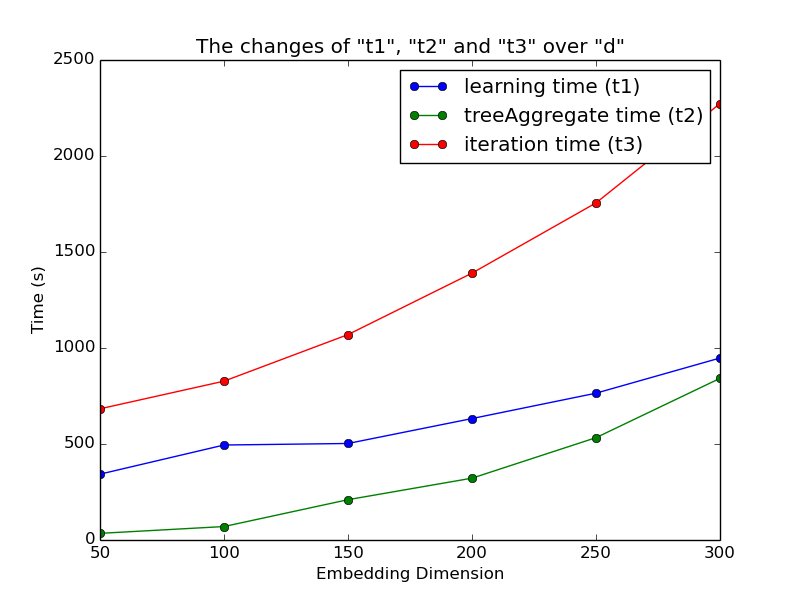
\includegraphics[width=0.75\textwidth]{vectime} 
	\caption{Shows the effect of varying embedding dimensionality of our model on the Time}
	\label{fig:vectime}
\end{figure}

\begin{figure}[tb]
  \centering
	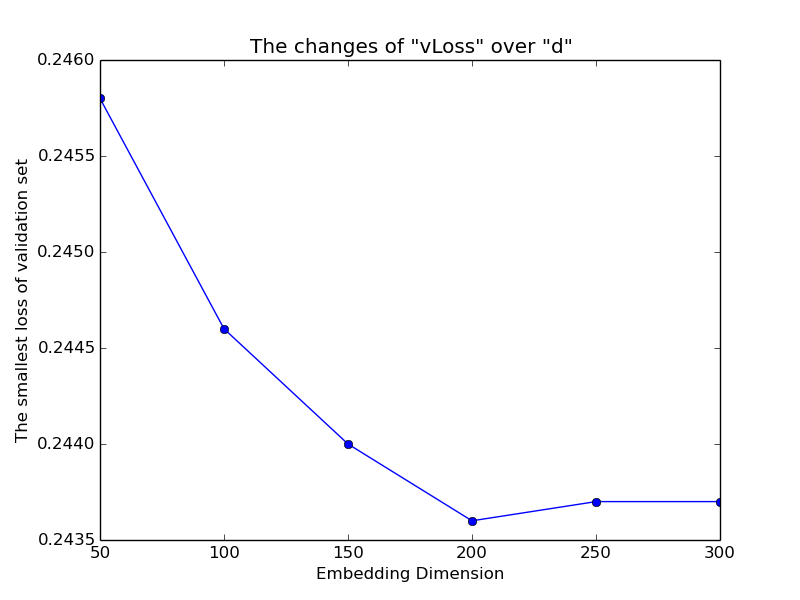
\includegraphics[width=0.75\textwidth]{vecloss} 
	\caption{Shows the effect of varying embedding dimensionality of our model on the loss of validation set}
	\label{fig:vecloss}
\end{figure}

\begin{figure}[!ht]
  \centering
	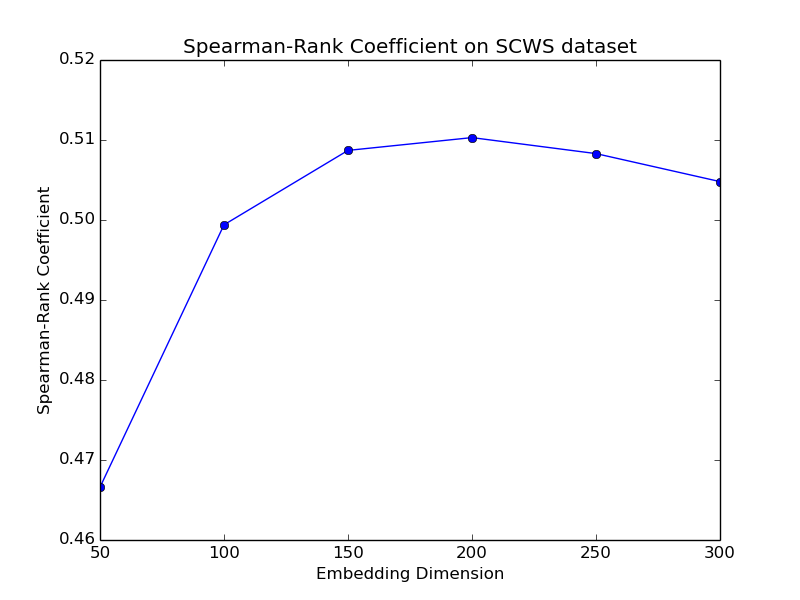
\includegraphics[width=0.75\textwidth]{vecSCWS} 
	\caption{Shows the effect of varying embedding dimensionality of our model on the SCWS task}
	\label{fig:vecSCWS}
\end{figure}


\begin{figure}[tb]
  \centering
	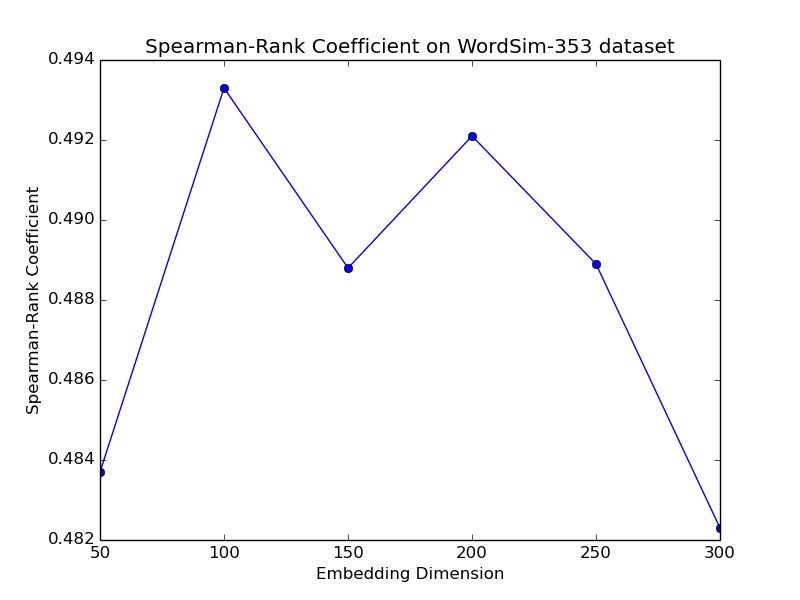
\includegraphics[width=0.75\textwidth]{vecword353} 
	\caption{Shows the effect of varying embedding dimensionality of our model on the WordSim-353 task}
	\label{fig:vecword353}
\end{figure}




\paragraph{Different Min Count} \ \\
We can find from Table \ref{tab:group2} that the size of dictionary is not the important factor. A higher $c1$ (minimal count for the inclusion of a word in vocabulary \gls{D}) remove some words from the vocabulary which are not frequent. As we know , each word's embedding vector is trained based on the surrounding words. Since those words are infrequent, each of them enters the training of frequent words only in a small amount. So they won't affect the final embedding vectors of frequent words. We think the above reason can also explain that their $iter$ (the total number of training iteration) is same. As we know $iter$ can imply the convergence speed. Removing infrequent words dose not influence the training of other words. 

For the similarity tasks, experiment 6 has obviously better score on both datasets. Its $c1$ is bigger, accordingly its dictionary size is smaller, so that it focuses on those more frequent words and can obtain more meaningful information (some infrequent words may affect the final result). And the time ($t1$, $t2$, $t3$ and $t4$) from experiment 13 is much more, because it has much bigger size of dictionary (5 times of one in experiment 6). As we know from the last chapter, we can also check the Figure \ref{fig:1to51} and Figure \ref{fig:51to637}: when $c1=20$, \gls{N} (the size of dictionary \gls{D}) is 458142; when $c2=200$, \gls{N} is 95434.

\begin{table}[tb]
\caption{Different Min Count Comparison} \label{tab:group2} 
\begin{center}
\begin{tabular}{|l|l|l|l|l|l|l|l|l|l|}
\hline
$id$& $c1$ & $t1$ & $t2$  & $t3$ & $t4$ & $iter$ & $loss$ & $SCWS$ & $word353$	   \\ 
\hline
6 	&  200 	& 342.9	& 34.6	& 683.3 &	23915  & 35 & 0.2458 &0.4666 & 0.4838  \\ 
\hline
13	&  20	& 849.0	& 343	& 1838.1 &	64335  & 35 & 0.2457 &0.4371	& 0.4293    \\ 
\hline
\end{tabular}
\end{center}
\end{table}

\clearpage % force tables/figures to be rendered

\paragraph{Different Sense Count Comparison} \ \\
From Table \ref{tab:group3}, we can know the sense count is not the most important factor to affect the final loss. And their similarity task scores are also similar. Figure \ref{fig:sensecount} shows the number of words for different number of senses per word.  Comparing the running time of these three experiments, we can find that the time ($t1$, $t2$, $t3$ and $t4$) from experiment $id=9$ are all less than the time from experiment $id=7$, because they have the same number of words with one sense but experiment 9 has fewer words with sense 3. Similarly, the time of experiment 10 is also less than experiment 7, because they have the same number of words with three senses but experiment 10 has fewer words with two senses. Actually, more senses means more parameters, and the experiment with fewer parameters is faster. For the loss and similarity task scores, the difference is not so clear to analysis. We think we can do some experiments with more different number of senses and try more senses for each word in the future to find out how different number of senses influence the loss and similarity task scores.

\begin{table}[tb]
\caption{Different Sense Count Comparison} \label{tab:group3} 
\begin{center}
\begin{tabular}{|l|l|l|l|l|l|l|l|l|l|l|}
\hline
$id$ & $c2$ & $c3$ & $t1$ & $t2$  & $t3$ & $t4$ & $iter$ &  $vLoss$  &  $SCWS$ & 	$word353$	   \\ 

\hline
13	& 2000 & 10000	& 849	& 343	& 1838 &	64335  & 35	& 0.2457 &0.4371	&0.4293	  \\ 
\hline
14 	& 2000 & 100000 	& 798	& 338	& 1712 &	59912  & 35	& 0.2465 &0.443 & 0.4375  \\ 
\hline
15 	& 7000 & 10000 	& 808	& 340	& 1740  &60909  & 35 & 0.2462 &0.4351 & 0.4412  \\ 
\hline
\end{tabular}
\end{center}
\end{table}


\begin{figure}[tb]
  \centering
	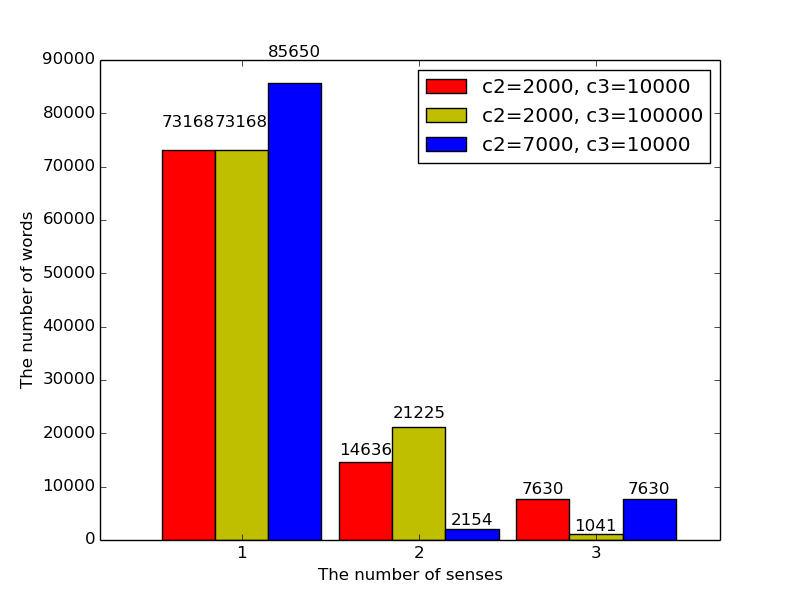
\includegraphics[width=1.0\textwidth]{sensecount} 
	\caption{Shows the number of words with different number of senses from three experiments}
	\label{fig:sensecount}
\end{figure}


\paragraph{Different Learning Rate and Gamma} \ 

Table \ref{tab:group41} and Table \ref{tab:group42} show that their time on one iteration ($t1$,$t2$ and $t3$) is almost same except the experiment 6 , which is very weird. The possible reasons about experiment 6 can be that we did experiment 6 earlier than other experiments and there may be some changes of hardware and environment which causes very different running time. 

For the learning rate $lr$ (the beginning learning rate) comparison, Figure \ref{fig:lrloss}, Figure \ref{fig:lriter} and Table \ref{tab:group41} tell us bigger $lr$ can get smaller $vLoss$ (the best loss of validation set) but requires more training iterations.

For the gamma $gm$ (the reduction factor of learning rate) comparison, Figure \ref{fig:gmloss}, Figure \ref{fig:gmiter} and Table \ref{tab:group42} show that bigger $gm$ can get smaller $vLoss$ (the best loss of validation set) but requires more training iterations.

In short, if we want to get smaller $vLoss$, we should increase both $lr$ and $gm$, but from above figures ( \ref{fig:lrloss}, \ref{fig:lriter}, \ref{fig:gmloss} and \ref{fig:gmiter} ), we can see that sometimes $vLoss$ reduces very few and $iter$ increases a lot. To balance the running time and the final loss, we select $lr=0.1$ and $gm=0.9$. 

\begin{table}[tb]

\caption{Different Learning Rate Comparison} \label{tab:group41} 
\begin{center}
\begin{tabular}{|l|l|l|l|l|l|l|l|l|}
\hline
$id$& $lr$ & $gm$ & $t1$ & $t2$  & $t3$ & $t4$ & $iter$ &    $vLoss$  	  \\ 
\hline
7   & 0.2 & 0.9 & 818.2  & 19.7  & 1416 &    63721  & 45 & 0.2445 \\ \hline
6 	& 0.1 & 0.9 & 342.9	& 34.6	& 683.3 &	23915  & 35 & 0.2458  \\ \hline 
8   & 0.05 & 0.9 & 789.1  & 18.4  & 1367 &   41013  & 30 & 0.2485 \\ \hline
9   & 0.01 & 0.9 & 745.7  & 19.0  & 1381 &   34516  & 25 & 0.2632  \\ \hline
\end{tabular}
\end{center}
\end{table}

\begin{table}[tb]
\caption{Different Gamma Comparison} \label{tab:group42} 
\begin{center}
\begin{tabular}{|l|l|l|l|l|l|l|l|l|}
\hline
$id$& $lr$ & $gm$ & $t1$ & $t2$  & $t3$ & $t4$ & $iter$ &    $vLoss$  	  \\ 
\hline
10   & 0.1 & 0.95 & 854.0  & 18.5  & 1402 &   77110  & 55 & 0.2443 \\ \hline
6 	& 0.1 & 0.9 & 342.9	& 34.6	& 683.3 &	23915  & 35 & 0.2458   \\ \hline
11   & 0.1 & 0.85 & 768.9  & 19.8  & 1413 &   42402  & 30 & 0.2476 \\ \hline
12   & 0.1 & 0.8 & 850.0  & 19.0  & 1479 &   36985  & 25 & 0.2490 \\ \hline
\end{tabular}
\end{center}
\end{table}

\begin{figure}[H]
\centering
        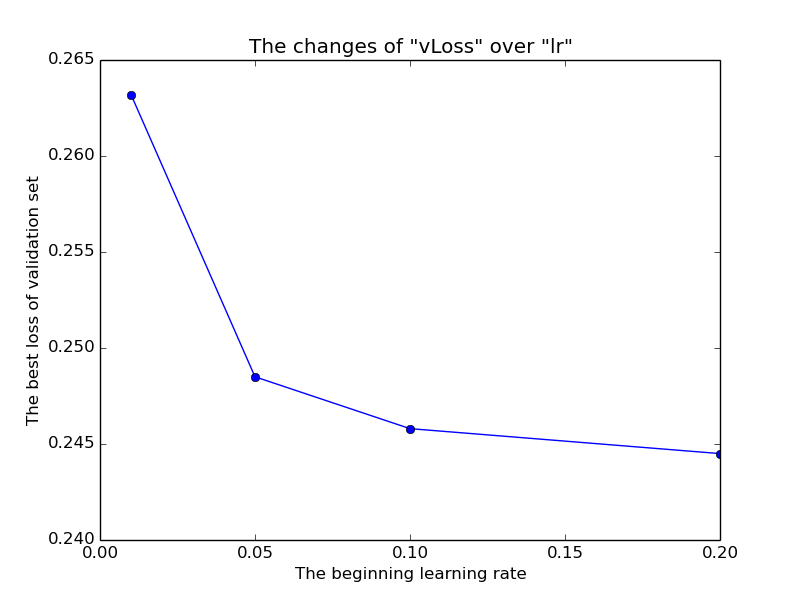
\includegraphics[width=0.75\textwidth]{lrloss} 
        \caption{Shows the effect of varying beginning learning rate on the best loss of validation set}	
        \label{fig:lrloss}
\end{figure}        

\begin{figure}[H]
\centering
        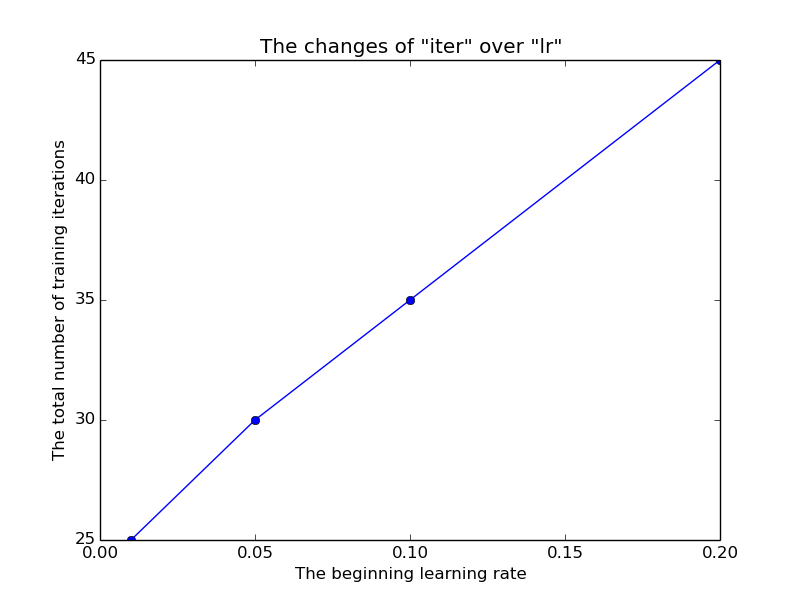
\includegraphics[width=0.75\textwidth]{lriter} 
		\caption{Shows the effect of varying beginning learning rate on the total number of training iterations}
		\label{fig:lriter}
\end{figure}

\begin{figure}[H]
\centering 
        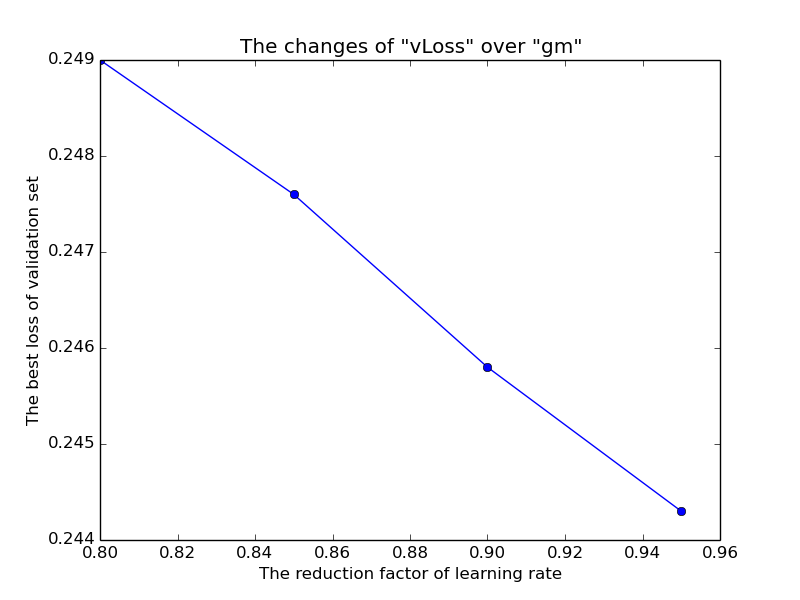
\includegraphics[width=0.75\textwidth]{gmloss} 	
        \caption{Shows the effect of reduction factor of the learning rate on the best loss of validation set}
        \label{fig:gmloss}
\end{figure}

\begin{figure}[H]
\centering 
        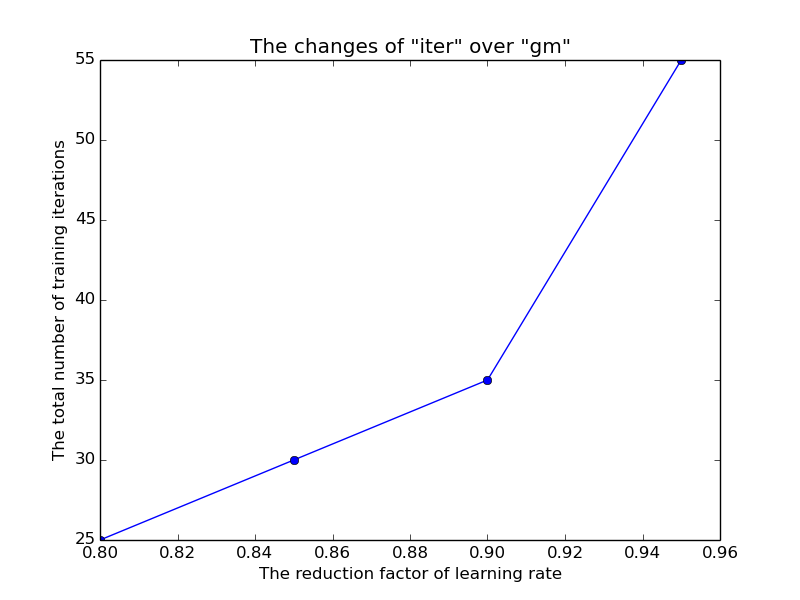
\includegraphics[width=0.75\textwidth]{gmiter} 
		\caption{Shows the effect of reduction factor of the learning rate on the total number of training iterations}
		\label{fig:gmiter}
\end{figure}

\paragraph{Different Number of Output Senses}  \ \\
From Table~\ref{tab:group5}, we can find that the difference in this group is very obvious comparing with previous groups. But $t2$ (the average time of collecting parameters in one iteration) is almost same. Actually in our program to be able to change the  number of output senses (one or multiple) easier, we do not change the data structure $syn1$ and let $syn1$ always have several embedding vectors for each word, if $S1=true$ the program only process the first embedding vector for each word. So these two experiments have the same number of parameters. And the time of collecting parameters is only influenced by the number of parameters, that's why their $t2$ is very similar. Note that $t1$ (the average time of learning parameters in one iteration) of experiment 16 is a little bigger than one of experiment 13  and $t3$ ( the average time of all operations in one iteration) of experiment 16 is much bigger than one of experiment 13. Multiple output embedding vectors for each word means more time to do sense assignment, specifically it requires more times of adjusting senses for each sentence to achieve stable, that's why $t3$ (including the time of sense assignment) is very different. In the process of learning parameters, no matter how many output senses, the the number of learning samples are same. So we can not tell the real reason about difference of $t1$. The possible reason can be from the program structure. We will analysis our program and do some testing experiments to find out the reason in the future. \com{changed}

The Table~\ref{tab:group5} also shows that the convergence speed of experiment 16 is slower (it has more training iterations) because it has several output senses and requires more iterations to adjust senses and learn embedding vectors. The $vLoss$ of experiment 16 is obviously smaller, because the fact of several output senses means more options for each center word to do prediction. It can make the final predicting probability based on the whole dataset bigger, which means smaller loss.  \com{added}

But we compare the nearest words for different senses of selected words from these two experiments in the Table \ref{tab:nearestcompare}. It is clear that if words can have multiple output embedding vectors (experiment 16), the nearest words of different senses for each word are similar, which can not achieve our goal. \com{added} After inspection the closest neighbors of senses the reason got clear. Say there are two words, e.g. "bank" and "money" with multiple senses. Then if money$_1$ was a close neighbor of bank$_0$ then it turned out that money$_0$ was a close neighbor of bank$_1$. Hence the closest senses were simply permuted, and the senses were not really meaningful. Hence we concluded that there should be only one output sense for each word. This will avoid this effect. 

\begin{table}[tb]

\caption{Comparison of the different number of output senses} \label{tab:group5} 
\begin{center}
\begin{tabular}{|l|l|l|l|l|l|l|l|l|l|}
\hline
$id$& $S1$ & $t1$ & $t2$ & $t3$ & $t4$ & $iter$ &    $vLoss$  	   \\ 
\hline
13	& true (one sense)		& 849	& 343	& 1838 &	64335 & 35& 0.2457 	   \\ 
\hline
16 	& false (multiple senses)& 1192	& 365	& 2866 &	128949 & 45& 0.2069  \\ 
\hline
\end{tabular}
\end{center}
\end{table}
 

\begin{table}[tb]
\caption{Nearest words comparison} \label{tab:nearestcompare} 

\begin{center}
\begin{tabular}{ |l|l|l| }
\hline
 & $id$ 13 , one sense output embedding& $id$ 16, multiple senses output embedding \\
\hline
\hline
\multirow{3}{*}{apple} 
 & cheap, junk, scrap, advertised 				& kodak, marketed, nokia, kit \\
 & chocolate, chicken, cherry, berry 		& portable, mgm, toy, mc \\
 & macintosh, linux, ibm, amiga			& marketed, chip, portable, packaging \\ 
 \hline
\multirow{3}{*}{bank} 
 & corporation, banking, banking, hsbc & trade, trust, venture, joint \\
 & deposit, stake, creditors, concession & trust, corporation, trade, banking \\ 
 & banks, side, edge, thames &  banks, border, banks, country \\ 
 \hline
\multirow{3}{*}{cell} 
 & imaging, plasma, neural, sensing & dna, brain, stem, virus \\
 & lab, coffin, inadvertently, tardis & cells, dna, proteins, proteins \\
 & cells, nucleus, membrane, tumor & dna, cells, plasma, fluid \\
\hline
\end{tabular}
\end{center}
\end{table}

\subsection{Comparison to prior analyses}

We fetch the results of similarity task scores from experiment 3 and experiment 6 to compare with other models in Table \ref{tab:SCWS} and Table \ref{tab:word353}. Table \ref{tab:word353} compares our model with Huang's model (\cite{HuangSocherEtAl2012}), the model from \citep{CollobertWeston2008} ($\mathrm{C}\&\mathrm{W}$), and the Skip-gram model \citep{MikolovSutskeverEtAl2013}, where $\mathrm{C}\&\mathrm{W}^*$ is trained without stop words. Our result is very bad on WordSim-353 task. Our model may not be suitable for word similarity task without context information. Table \ref{tab:SCWS} compares our model with Huang's model \citep{HuangSocherEtAl2012} , and the models from \citep{NeelakantanShankarEtAl2015} (MSSG and NP-MSSG). The number after the model name is the embedding dimension, i.e. MSSG-50d means MSSG model with 50 embedding dimension. 

Even that our score on SCWS is still not good.  The possible reasons can be that our model do not remove the stop words, we do not use sub-sampling used word2vec (\cite{MikolovSutskeverEtAl2013}),  our training is not enough and we uses too many executors (32 cores), where fewer executors may give us better results. Additionally, we only use $localSim$ and $avgSim$ for SCWS task and $avgSim$ for WordSim-353 task, which may not be suitable for our model. We will try other similarity functions. From Tabel \ref{tab:SCWS}, we can see NP-MSSG performs really good on SCWS task. We think we can also follow some idea from it and improve our model in the future so that the model can have dynamic number of senses.



\begin{table}
\caption{Experimental results in the SCWS task. The numbers are Spearmans correlation $\rho$ $\times$ 100} \label{tab:SCWS} 
\begin{center}
\begin{tabular}{|l|l|l|}
\hline
Model & avgSim & localSim  \\ 
\hline
Our Model-50d & 55.8 & 46.7 \\
\hline
Our Model-300d & 56.9 & 50.5	\\ 
\hline
Huang et al-50d  & 62.8	& 26.1 \\ 
\hline
MSSG-50d  & 64.2	 & 49.17 \\ 
\hline
MSSG-300d  & 67.2 & 57.26 \\ 
\hline
NP-MSSG-50d  & 64.0 & 50.27 \\ 
\hline
NP-MSSG-300d  & 67.3 & 59.80 \\ 
\hline
\end{tabular}
\end{center}
\end{table}


\begin{table}
\caption{Results on the WordSim-353 dataset} \label{tab:word353} 
\begin{center}
\begin{tabular}{|l|l|}
\hline
Model & $\rho$ $\times$ 100 \\ 
\hline
Our Model-50d &  48.4 \\
\hline
Our Model-300d & 48.2	\\ 
\hline
$\mathrm{C}\&\mathrm{W}^*$  	& 49.8\\ 
\hline
$\mathrm{C}\&\mathrm{W}$ 	& 55.3\\ 
\hline
Huang et al 	& 64.2\\ 
\hline
Skip-gram-300d  	& 70.4\\ 
\hline
\end{tabular}
\end{center}
\end{table}
 
 



 
\section{Case Analysis}

\begin{table}[tb]
	\caption{Sense Similarity Matrix of $apple$} \label{tab:sensematrixapple} 
	\begin{center} \begin{tabular}{|l|l|l|l|}  
			\hline
			& $apple_0$ & $apple_1$ & $apple_2$ \\ 
			\hline  
			$apple_0$  & 1.000000  & 0.788199 & 0.800783 \\ 
			\hline 
			$apple_1$  & 0.788199 & 1.000000 & 0.688523  \\ 
			\hline 
			$apple_2$  & 0.800783 & 0.688523 & 1.000000  \\
			\hline
		\end{tabular} 
	\end{center}
\end{table}
In the following, we will select only one experiment's result to do the visualization of senses and compute nearest word senses. The selection is based on the final loss and similarity task, specifically it is experiment 13 from above.   

\begin{table}[tb]
	
	\caption{Nearest Words of $apple$} \label{tab:nearestapple} 
	\begin{center} \begin{tabular}{|l|l|}  
			\hline 
			$apple_0$: & cheap , junk , scrap , advertised , gum , liquor , pizza   \\  
			\hline
			$apple_1$: & chocolate, chicken, cherry, berry, cream, pizza, strawberry  \\  
			\hline
			$apple_2$: & macintosh, linux, ibm, amiga, atari, commodore, server   \\  
			\hline
		\end{tabular}
	\end{center}
\end{table}

Firstly we give the result for the word $apple$, where different sense are quite nicely separated. Table \ref{tab:sensematrixapple} shows the sense similarity matrix of $apple$. The similarity value is the cosine similarity between two embedding vectors. Table \ref{tab:nearestapple} shows the nearest words of different senses from $apple$. We can see that $apple_0$ and $apple_1$ are about food. They are similar somehow. And $apple_2$ is about the computer company. The next are some sentence examples including the word $apple$ in Table \ref{tab:sentenceapple}. These are the sentences containing the assigned word senses from the last iteration of training. To make it clear, we only display the sense label of the $apple$, although the other words also have multiple senses.

To visualize semantic neighborhoods we selected 100 nearest words for each sense of $apple$ and use t-SNE algorithm \citep{MaatenHinton2008} to project the embedding vectors into two dimensions. And then we only displayed $70\%$ of words randomly to make visualization better, which is shown in Figure \ref{fig:apple}. 
 


\begin{table}[tb]

\caption{Sentence Examples of $apple$} \label{tab:sentenceapple} 
\begin{center} 
\begin{tabular}{|l|l|}
\hline
\multirow{2}{*}{$apple_0$} 
&he can't tell an onion from an \textcolor{red}{$apple_0$} and he's your eye witness\\
&some fruits e.g \textcolor{red}{$apple_0$} pear quince will be ground\\
\hline
\multirow{2}{*}{$apple_1$} 
&the cultivar is not to be confused with the dutch rubens \textcolor{red}{$apple_1$}\\
&the rome beauty \textcolor{red}{$apple_1$} was developed by joel gillette \\
\hline
\multirow{2}{*}{$apple_2$} 
&a list of all \textcolor{red}{$apple_2$} internal and external drives in chronological order\\
&the game was made available for the \textcolor{red}{$apple_2$} iphone os mobile platform\\
\hline
\end{tabular} 
\end{center}
\end{table}


\begin{figure}[tb]
	\caption{Nearest words from $apple$}
  \centering
	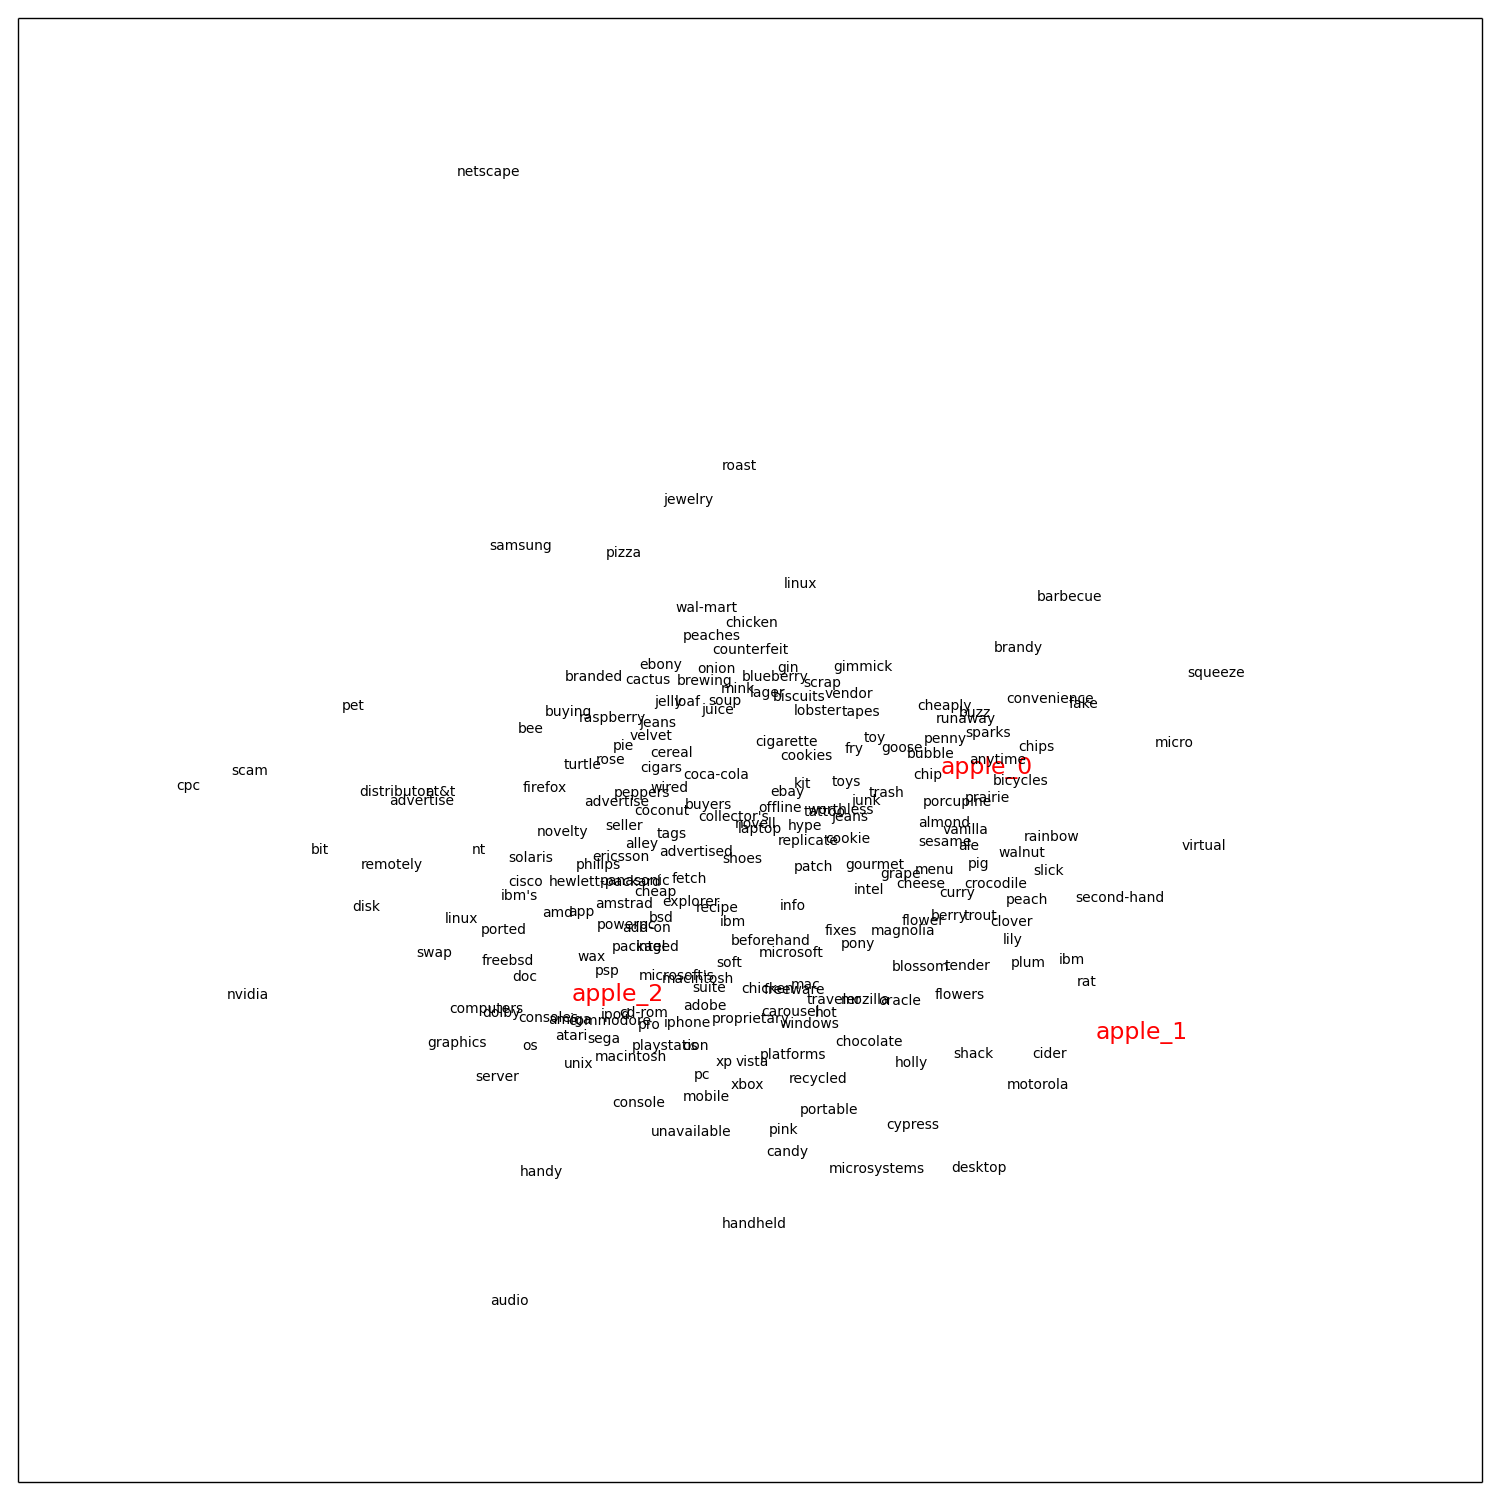
\includegraphics[width=1.0\textwidth]{apple} 
	\label{fig:apple}
\end{figure}

\clearpage % force floats to be dislayed

\paragraph{} Next, we select other 5 words $fox$ , \ $net$ , \ $rock$ , \ and $plant$, and list nearest words to each of their 3 senses in Table \ref{tab:nearestwordsother}. Each line contains the nearest words for one of the senses. This table nicely illustrates the different meanings of words: 
\begin{itemize}
	\item fox: Sense 1 and 2 cover different movies and film directors while sense 3 is close to tv networks.
	\item net: Sense 1 is related to communication networks, sense 2 to profits and earnings and sense 3 to actions
	\item rock: Sense 1 and sense 2 is related to music while sense 3 to stone.
	\item run: Sense 1 is related to election campains, sense 2 expresses the movement and sense 3 to public transport.
	\item plant: Sense 1 is close to biologic plants and small animals, sense 2 is related to flowers and sense 3 to factories.
\end{itemize}


In table \ref{tab:sentenceother} we show one example sentence for each sense.
The example sentences are also cut by ourself without affecting the meaning of the sentence. 


\begin{table}[tb]
\caption{Nearest words from $fox$ , \ $net$ , \ $rock$ , \ $run$ and \ $plant$} \label{tab:nearestwordsother} 
\begin{center} 
\begin{tabular}{|l|l|}
\hline
\multirow{3}{*}{$fox$}   
& archie, potter, wolfe, hitchcock, conan, burnett, savage  \\ 
& buck, housewives, colbert, eastenders, howard, kane, freeze
 \\ 
& abc, sky, syndicated, cw, network's, ctv, pbs \\ 
\hline
\multirow{3}{*}{$net$}  
& generates, atm, footprint, target, kbit/s, throughput, metering   \\  
& trillion, rs, earnings, turnover, gross, euros, profit  \\  
&jumped, rolled, rebound, ladder, deficit, snapped, whistle   \\  
\hline 
\multirow{3}{*}{$rock$}  
&echo, surf, memphis, strawberry, clearwater, cliff, sunset  \\  
& r$\,$b, hip, roll, indie, ska, indie, hop  
 \\  
&formations, crust, melting, lava, boulders, granite, dust   \\  
\hline 
\multirow{3}{*}{$run$}
& blair, taft, fraser, monroe, precinct, mayor's, governor's  \\  
& streak, rushing, tying, shutout, inning, wicket, kickoff
 \\  
& running, tram, travel, express, trams, inbound, long-distance \\
\hline  
\multirow{3}{*}{$plant$}
& plants, insect, seeds, seed, pollen, aquatic, organic  \\  
& flowering, orchid, genus, bird, species, plants, butterfly
 \\  
& electricity, steel, refinery, refinery, manufacturing, gas, turbine  \\
\hline
\end{tabular}
\end{center}
\end{table}


\begin{table}[tb]
\caption{Sentence Examples of $fox$ , \ $net$ , \ $rock$ , \ $run$ and \ $plant$ } \label{tab:sentenceother} 
\begin{center} 
\begin{tabular}{|l|l|}
\hline
\multirow{3}{*}{$fox$} 
&run by nathaniel mellors dan \textcolor{red}{$fox_0$} andy cooke and ashley marlowe\\
&he can box like a \textcolor{red}{$fox_1$} he's as dumb as an ox\\
&the grand final was replayed on fox sports australia and the \textcolor{red}{$fox_2$} footy channel\\
\hline
\multirow{3}{*}{$net$} 
&\textcolor{red}{$net_0$} supports several disk image formats partitioning schemes\\
&in mr cook was on the forbes with a \textcolor{red}{$net_1$} worth of billion \\
&nothin but \textcolor{red}{$net_2$} freefall feet into a net below story tower\\
\hline
\multirow{3}{*}{$rock$} 
&zero nine is a finnish hard \textcolor{red}{$rock_0$} band formed in kuusamo in\\
&matt ellis b december is a folk \textcolor{red}{$rock_1$} genre singer-songwriter\\
&cabo de natural park is characterised by volcanic \textcolor{red}{$rock_2$} formations\\
\hline
\multirow{3}{*}{$run$} 
&dean announced that she intends to \textcolor{red}{$run_0$} for mayor again in the november election\\
& we just couldn't \textcolor{red}{$run_1$} the ball coach tyrone willingham said\\
& the terminal is \textcolor{red}{$run_2$} by british rail freight company ews\\
\hline
\multirow{3}{*}{$plant$} 
&these phosphoinositides are also found in \textcolor{red}{$plant_0$} cells with the exception of pip\\
&is a genus of flowering \textcolor{red}{$plant_1$} in the malvaceae sensu lato\\
&was replaced with a new square-foot light fixture \textcolor{red}{$plant_2$} in sparta tn\\
\hline
\end{tabular} 
\end{center}
\end{table}


\paragraph{} Finally, for each sense of each word ($apple$, $fox$, $net$, $rock$ and $plant$), we select only the 20 nearest words, and combine them together to do another t-SNE embeddingof  two dimensions. The the result is shown in Figure \ref{fig:keywords20}. 

\begin{figure}[tb]
  \centering
	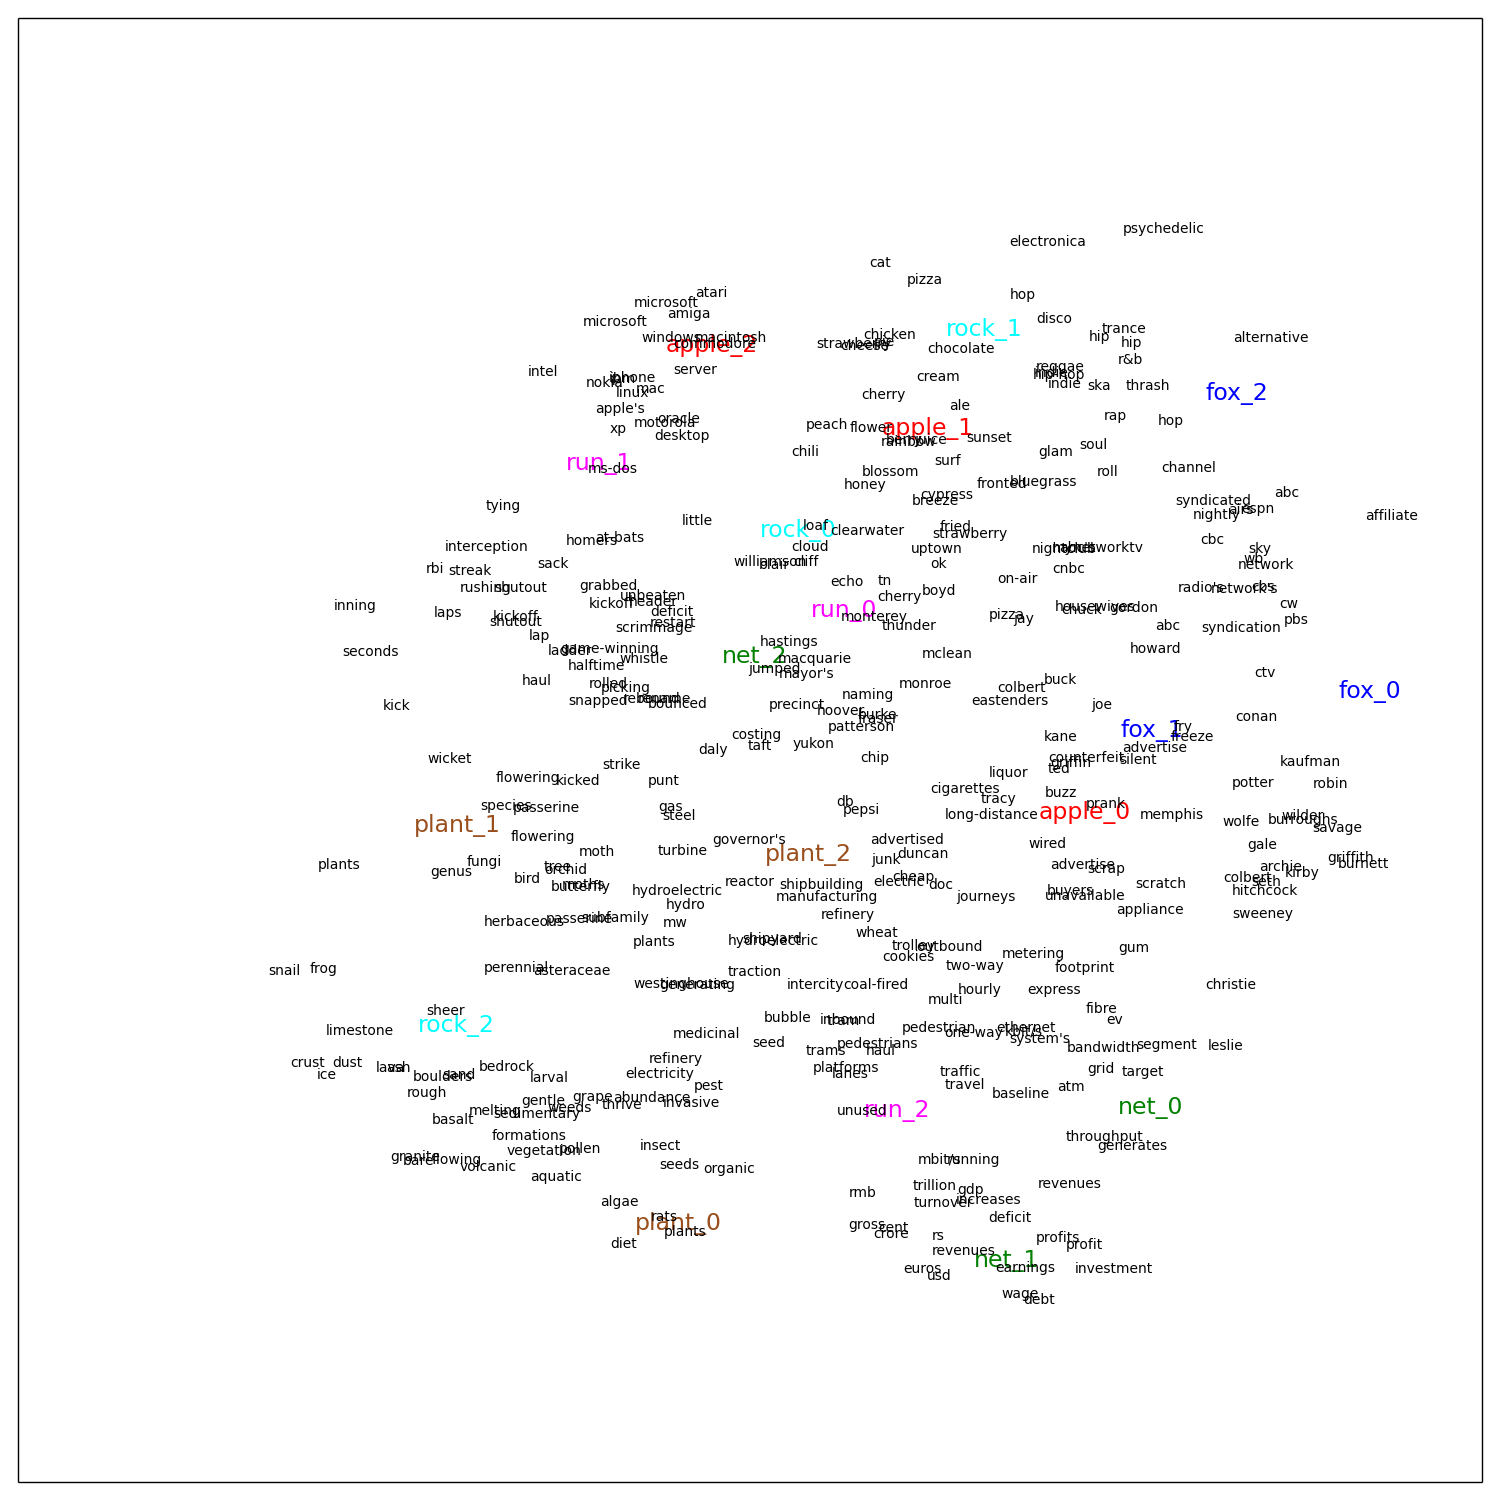
\includegraphics[width=1.0\textwidth]{some20} 
	\caption{Nearest words from $apple$,\ $fox$,\ $net$,\ $rock$,\ $run$ and $plant$}
	\label{fig:keywords20}
\end{figure}

\paragraph{} From these visualization, we can say our model is able to extract meaningful sense vectors which may be used for subsequent analyses. There is, however, room for improvement.
